%MÁSTER UNIVERSITARIO EN GESTIÓN SOSTENIBLE DE LA TIERRA Y EL TERRITORIO
%TÉCNICAS DE ANÁLISIS CUANTITATIVAS Y CUALITATIVAS
%DOCUMENTO DE RESOLUCIÓN DEL EJERCICIO 4 DE EVALUACIÓN
%MARCOS RIAL DOCAMPO


\documentclass[11pt,a4paper]{article}

\usepackage[utf8]{inputenc}
\usepackage[spanish]{babel}
\usepackage{amsmath}
\usepackage{amsfonts}
\usepackage{amssymb}
\usepackage{url}
\usepackage[colorlinks,linktocpage=true,citecolor=blue,linkcolor=blue]{hyperref}
\usepackage{booktabs}
\usepackage{graphicx,geometry}
\usepackage{caption}
\usepackage{verbatim,moreverb}

\usepackage{listings}
\lstset{
	frame=tb,
    framerule=0pt,
    aboveskip=3mm,
    belowskip=3mm,
    framextopmargin=3pt,
    framexbottommargin=3pt,
    %framexleftmargin=0.2cm,
    framesep=0pt,
    rulesep=.4pt,
    backgroundcolor=\color{gray97},
    rulesepcolor=\color{black},
    stringstyle=\color{mauve},
    showstringspaces = false,
    basicstyle=\footnotesize\ttfamily,
    commentstyle=\color{dkgreen},
    keywordstyle=\color{blue},
    numbers=left,
    numbersep=-6.5pt,
    numberstyle=\tiny\color{gray},
    numberfirstline = false,
    breaklines=true,
    morekeywords={*,...}
   }

\usepackage{xcolor}
\definecolor{gray97}{gray}{.97}
\definecolor{gray75}{gray}{.75}
\definecolor{gray45}{gray}{.45}
\definecolor{mauve}{rgb}{0.58,0,0.82}
\definecolor{dkgreen}{rgb}{0,0.6,0}

\author{Marcos Rial Docampo}
\title{Técnicas de Análisis Cuantitativas y Cualitativas\\Resolución del ejercicio de evaluación 4}
\date{\small{\today}}

\begin{document}
\maketitle

Disponemos de datos de los tiempos obtenidos por los participantes de una carrera popular. Se trata de 80 muestras de un total de 1140 que están estratificadas por sexo y categoría de edad.

Mediante un test de Shapiro-Wilk comprobamos si la variable \textit{total.minutos} tiene una distribución normal. Para ello podemos aplicar el test a todas las observaciones de la variable o dividirla en grupos. En este caso dividiremos la variable en los cuatro grupos correspondientes a la categoría de la prueba (infantil-cadete, junior, senior y veteranos), pero podríamos haberlo hecho por sexo o por subcategoría. Obtenemos los resultados mostrados en el cuadro \ref{tab:Shapiro} y los gráficos de la figura \ref{fig:diagrama} donde se indica que la variable \textit{total.minutos} tiene una distribución normal en cada uno de los grupos de edad.

\begin{table}[ht]
\centering
\begin{tabular}{cr@{,}lr@{,}l}
\toprule[0.4mm]
\multicolumn{5}{c}{Test Shapiro-Wilk}\\
 & \multicolumn{2}{c}{W} & \multicolumn{2}{c}{p-valor}\\
\midrule
Infantil-Cadete & 0&93455 & 0&1888\\
Junior & 0&93301 & 0&1765\\
Senior & 0&96890 & 0&7315\\
Veterano & 0&96757 & 0&7029\\
\bottomrule[0.4mm]
\end{tabular}
\captionsetup{font={footnotesize,it}}
\caption{Resultado del test de Shapiro-Wilk para la variable ``total.minutos''.}
\label{tab:Shapiro}
\end{table}

\begin{figure}
\centering
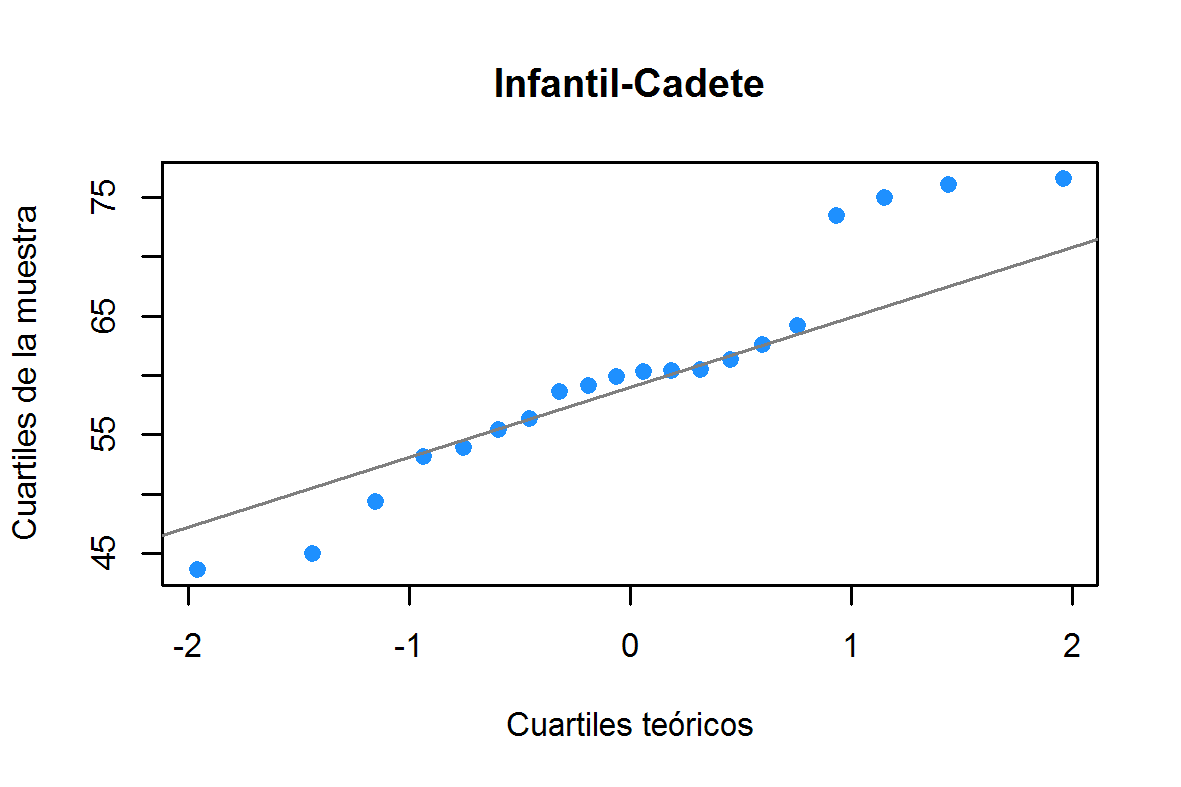
\includegraphics[scale=0.725]{./R/Graficos/CuartInfantil.png}
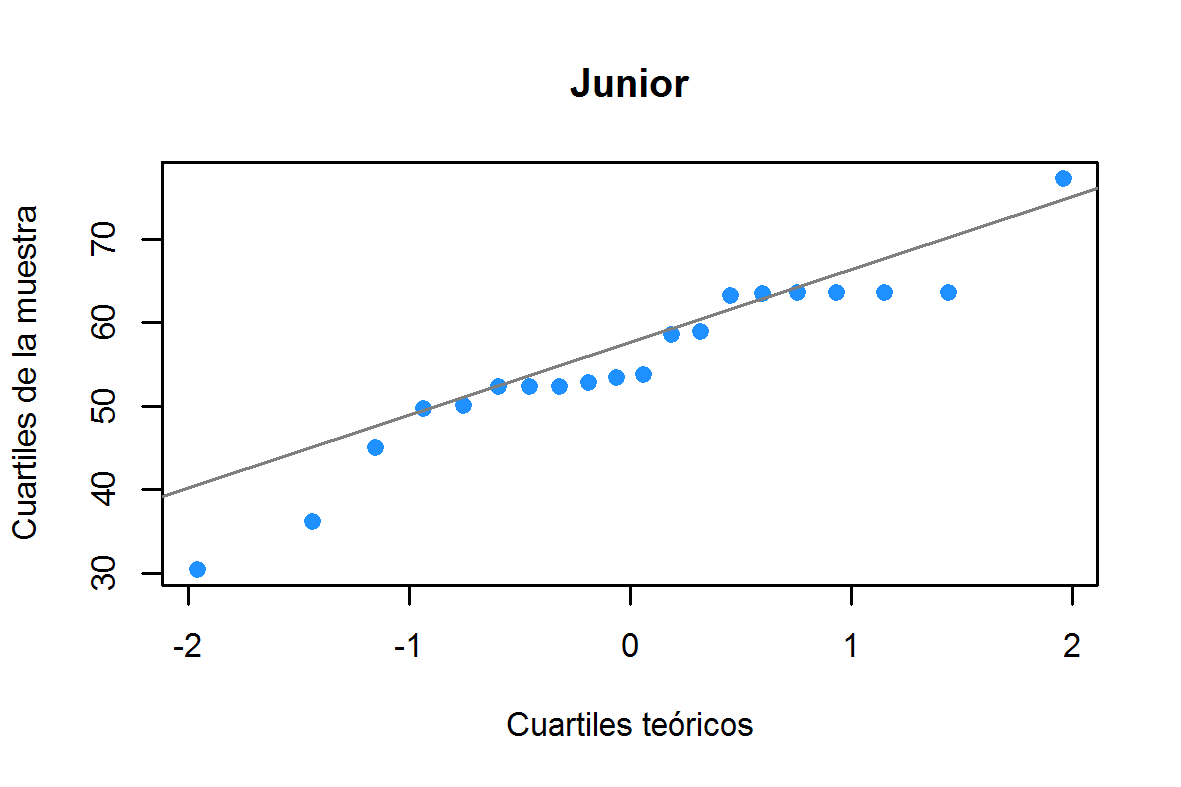
\includegraphics[scale=0.725]{./R/Graficos/CuartJunior.png}
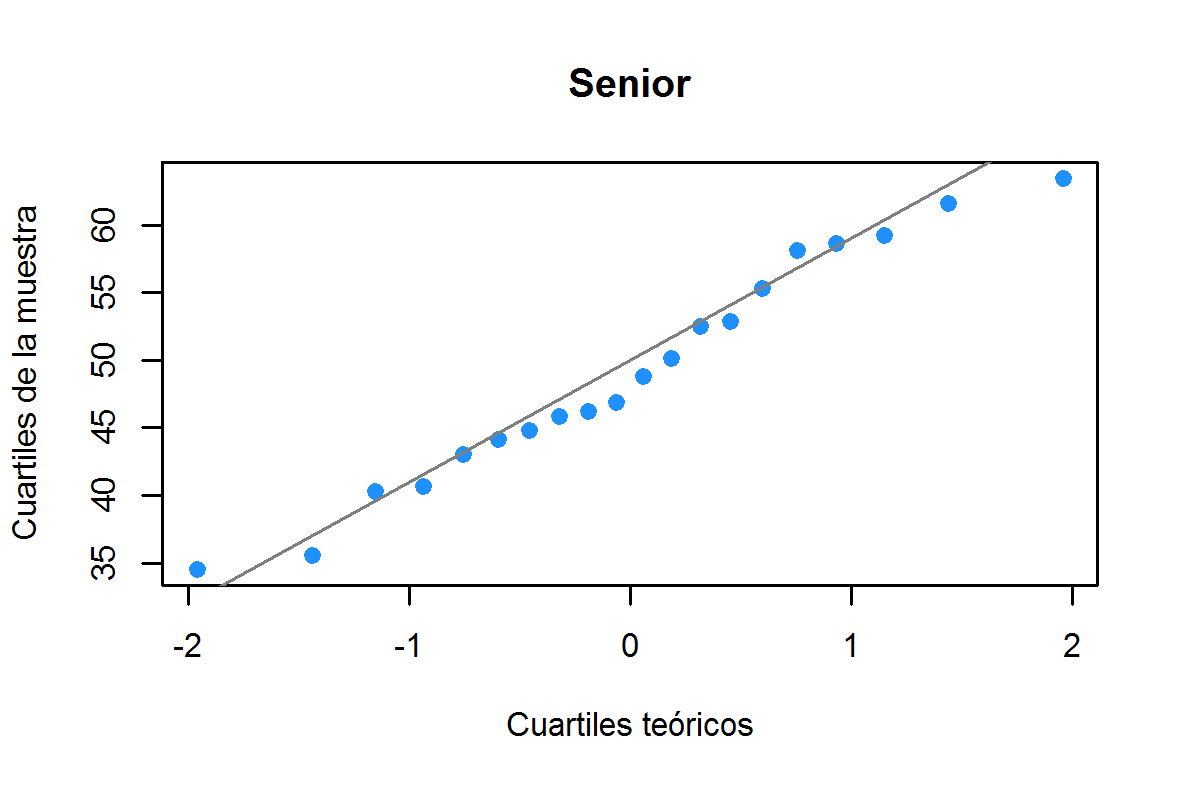
\includegraphics[scale=0.725]{./R/Graficos/CuartSenior.png}
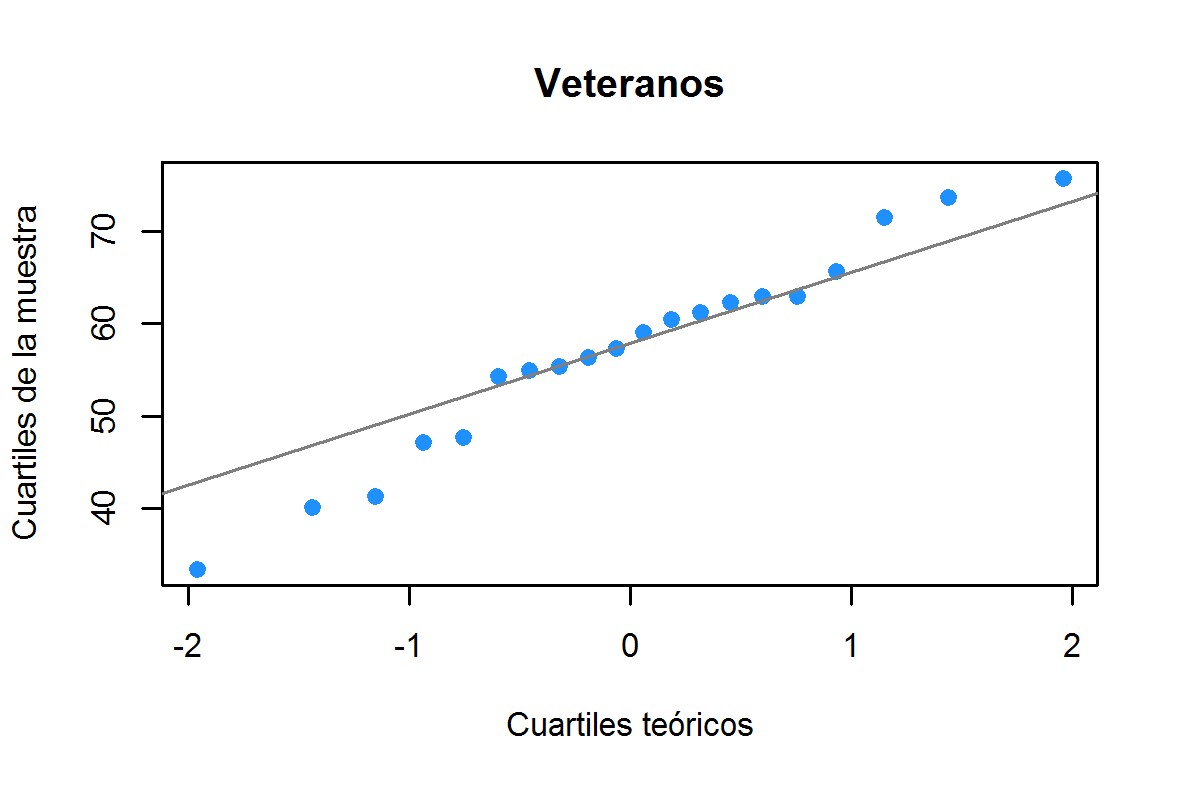
\includegraphics[scale=0.725]{./R/Graficos/CuartVeteranos.png}
\captionsetup{font={footnotesize,it}}
\caption{Diagramas de cuartiles para las categorías de la muestra.}
\label{fig:diagrama}
\end{figure}

Es interesante saber si la variable sexo tiene influencia sobre los tiempos obtenidos por los participantes de la prueba. Al ser el sexo de los participantes un factor de dos niveles, podemos realizar un contraste de hipótesis mediante un test de Welch. Obtenemos los resultados del cuadro \ref{tab:sexo} y la figura \ref{fig:boxsexo} donde vemos que la media del tiempo empleado por las mujeres es casi 9 minutos superior al de los hombres. Además, un p-valor de 7,405e$^{-05}$ sugiere que la interpretación anterior de la diferencia de las medias es correcta. Realizando un análisis de varianza de un factor habríamos obtenido un resultado similar.

\begin{table}[ht]
\centering
\begin{tabular}{cc}
\toprule[0.4mm]
Sexo & Tiempo empleado (minutos)\\
\midrule
Femenino & 59,93\\
Masculino & 50,96\\
\bottomrule[0.4mm]
\end{tabular}
\captionsetup{font={footnotesize,it}}
\caption{Resultados de las medias de tiempo por sexo de los participantes en la prueba.}
\label{tab:sexo}
\end{table}

\begin{figure}
\centering
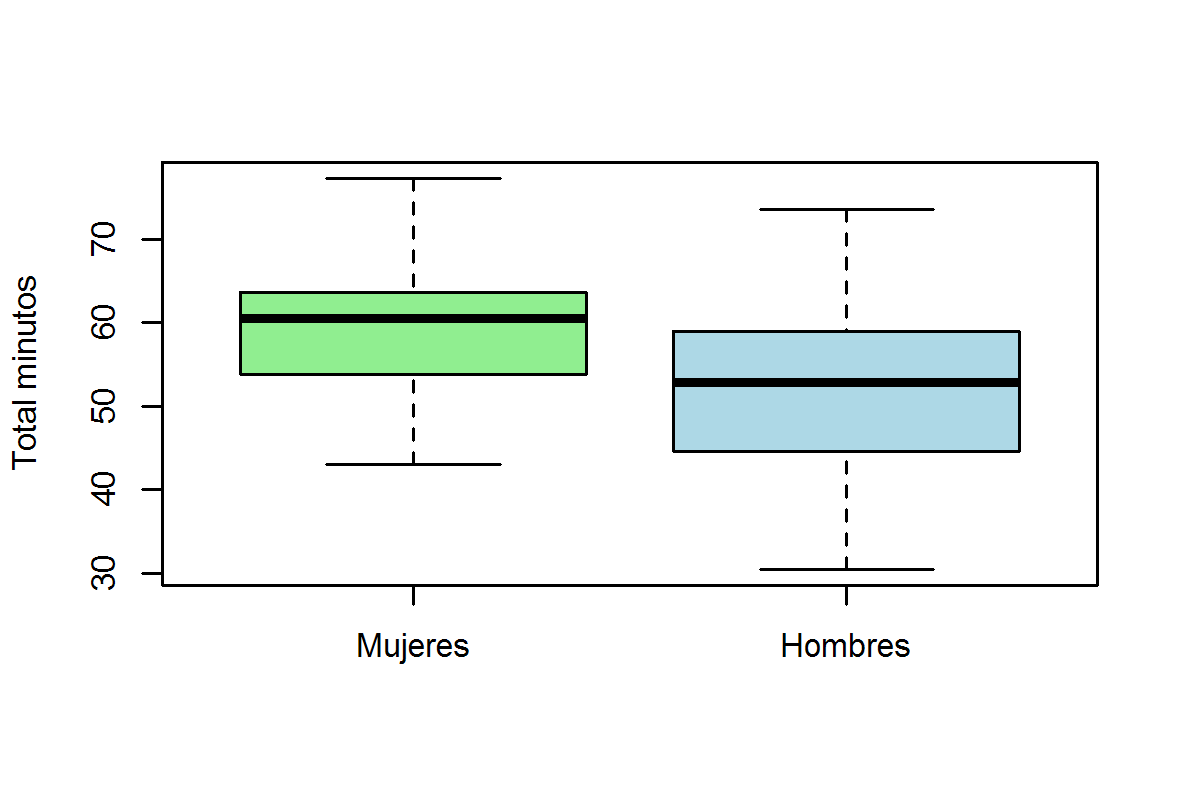
\includegraphics{./R/Graficos/Boxsexo.png}
\captionsetup{font={footnotesize,it}}
\caption{Representación gráfica de la diferencia en tiempos respecto al sexo de los participantes.}
\label{fig:boxsexo}
\end{figure}

Analizamos ahora la influencia que tienen los factores sexo y categoría sobre la variable tiempo en minutos. Primero analizamos la influencia de los dos factores por separado con una hipótesis nula (H$_{0}$) de que no afectan estos factores a los tiempos obtenidos por los participantes. Obtenemos los resultados del cuadro \ref{tab:anova1} donde vemos que ambos factores influyen por separado en los tiempos de la prueba deportiva.

\begin{table}[ht]
\centering
\begin{tabular}{cc}
\toprule[0.4mm]
Factor & Pr($>$F)\\
\midrule
Sexo & 2,09e$^{-05}$\\
Categoría & 0,0016\\
\bottomrule[0.4mm]
\end{tabular}
\captionsetup{font={footnotesize,it}}
\caption{Resultado del análisis de varianza para los factores sexo y categoría.}
\label{tab:anova1}
\end{table}

Una vez analizados por separado procedemos a hacerlo conjuntamente teniendo en cuenta la interacción de ambos factores. En este caso el resultado que nos da es que conjuntamente no afectan al tiempo total de los participantes. Con un Pr($>$F) obtenido de 0,2478 aceptamos la H$_{0}$. Observamos en la gráfica de interacción de la figura \ref{fig:interaccion1} que efectivamente los tiempos obtenidos por participantes femeninos están por encima de los masculinos en todas las categorías. En cambio en las categorías los tiempos se mezclan en cuanto al sexo como se muestra en la figura \ref{fig:interaccion2} en la categoría de veteranos.

\begin{figure}
\centering
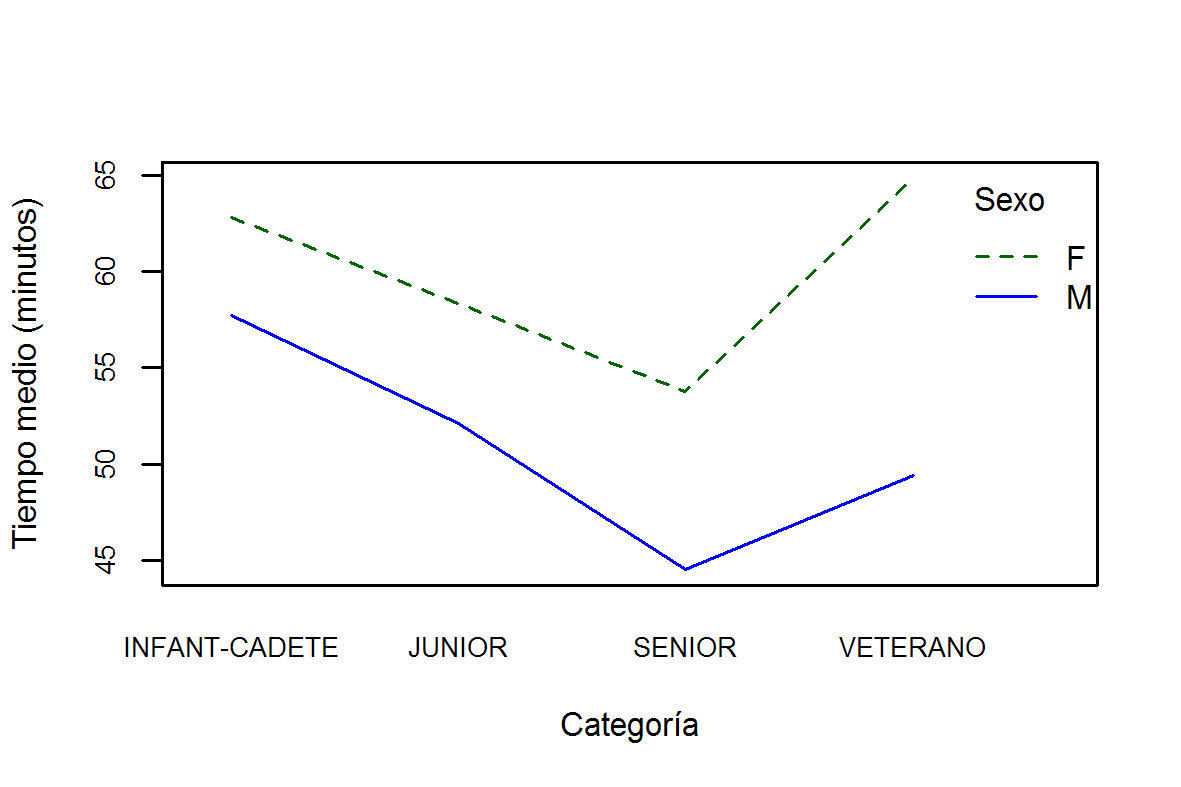
\includegraphics{./R/Graficos/Interaccion1.png}
\captionsetup{font={footnotesize,it}}
\caption{Gráfica de interacción entre los factores sexo y categoría con el tiempo de los participantes.}
\label{fig:interaccion1}
\end{figure}

\begin{figure}
\centering
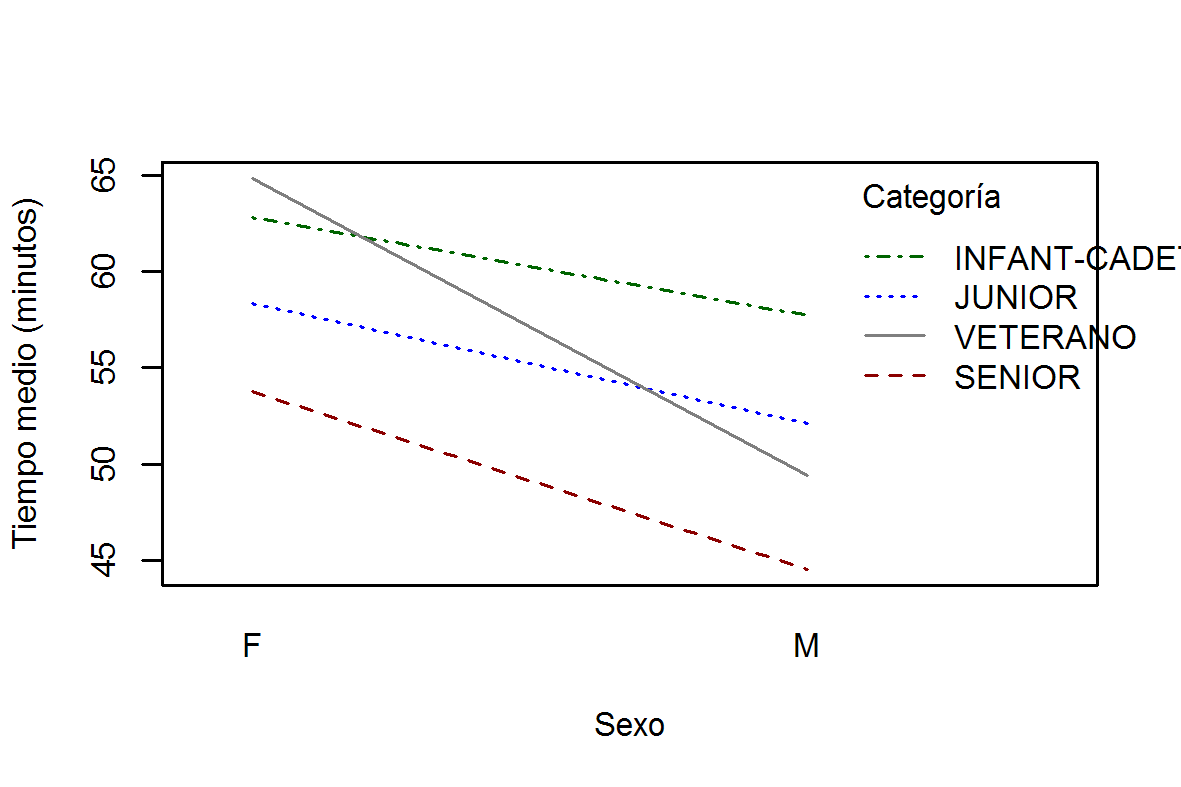
\includegraphics{./R/Graficos/Interaccion2.png}
\captionsetup{font={footnotesize,it}}
\caption{Gráfica de interacción entre los factores categoría y sexo con el tiempo de los participantes.}
\label{fig:interaccion2}
\end{figure}

Mediante un test de varianzas comprobamos la igualdad de estas para cada factor. Es decir, que gracias a este test y con una H$_{0}$ igual a que los factores estudiados presentan varianzas iguales comprobaremos la condición de homocedasticidad de estos con la variable \textit{total.minutos}.

Para el caso del factor sexo esta condición de homocedasticidad se cumple ya que el test devuelve un p-palor de 0,8756. En el caso de las categorías y aplicando un test de Bartlett (debido a que este factor tiene más de dos niveles) el resultado también nos dice que existe homocedasticidad con un p-valor de 0,6638.
\end{document}